\documentclass[11pt, titlepage]{article}
\usepackage{amsmath,amsthm,amssymb}
\usepackage{hyperref, pgf, tikz}
\usepackage{fancyhdr}
\usetikzlibrary{arrows}
\usepackage[margin=1.25in]{geometry}
\usepackage{graphicx}                     
\pagestyle{fancy}
\usepackage{array}
%\usepackage{wrapfig}

\lhead{Lab \#3}
\rhead{\thepage}
\cfoot{}

\title{The Addition and Resolution of Vectors: The Force Table\ \ \\ \large Lab \#3}
\author{Name: Avery Karlin \\ Partner: Alon Levin}
\date{}
\begin{document}

\maketitle

\begin{center}
\LARGE The Addition and Resolution of Vectors: The Force Table
\end{center}

\section*{Objective}
The objective of the lab is to graphically, mathematically, and experimentally add vectors, and compare the results of the methods.
\section*{Introduction}
Vectors are quantities with both magnitude and direction, such that they need more complicated methods of adding up than scalars (quantities with only magnitude).

The most obvious method of vector addition is done by graphing the vectors, head-to-tail, such that the vector from the first tail to the final head is the resultant vector, called the triangle method. A similar method places them tail to tail, forming two sides of a parallelogram, such that the diagonal of the resultant parallelogram from the vertex of the vectors is the resultant. The final similar graphical method uses a polygon, similar to the triangle method, head to tail for more than two vectors, such that the resultant vector is from the first tail to the final head.

The next common method of vector is analytical/mathematical means, by which the component vectors along each of the axises are found, such that for $\vec{r}$, $\vec{r_x} = \vec{r}cos(\theta)$ and $\vec{r_y} = \vec{r}sin(\theta)$, after which the x and y component of each vector are added up toproduce the components of the resultant vector. To put that vector in $(r, \theta)$ form, $r = \sqrt{r_x^2 + r_y^2}$ by the pythagorean theorem and $\theta = tan^{-1}(\frac{r_y}{r_x})$.

Mathematically, vectors can also be added up by the triangle method, placing them with the resultant in a triangle, head-to-tail, similar to the graphical method. By the law of cosines, $R_{result} = \sqrt{R_1^2 + R_2^2 - 2R_1R_2cos(\phi)}, where \phi is the angle between the vectors when placed head to tale$, after which the angle can be determined by the law of sines, such that $\frac{sin(\theta)}{R_2} = \frac{sin(\phi)}{R_{result}}$.

\section*{Procedures and Results}
Vector addition can also be done experimentally by a force table, such that strings are put at specific angles on the table, with a weight attached to signify the magnitude. These are then hooked to a ring at the center of the table, after which another vector is attached such that the ring moves to be perfectly centered on the table. This vector is the equlibriant vector, or the vector equal and opposite the sum of the two other vectors to balance them out, such that the sum of all three is zero. We can thus use that, reversing it, such that the angle is $180^o$ more, to find the resultant vector.

The equilibriant vector can be found by trial and error, approximating the correct angle such that the ring is centered perpendcular to the added vector, then using trial and error to determine the mass such that it is fully centered on the table.

For the vector resolution trial on the other hand, rather than getting vectors and finding the equilibriant, we are given a single vector, finding the component of the equilibriant on both the x and y axises ($0/180^o$ and $90/270^o$), using trial and error to determine the points such that it it is fully centered similarly.

\begin{figure}[p]
\centering
\hspace*{-10.5cm}
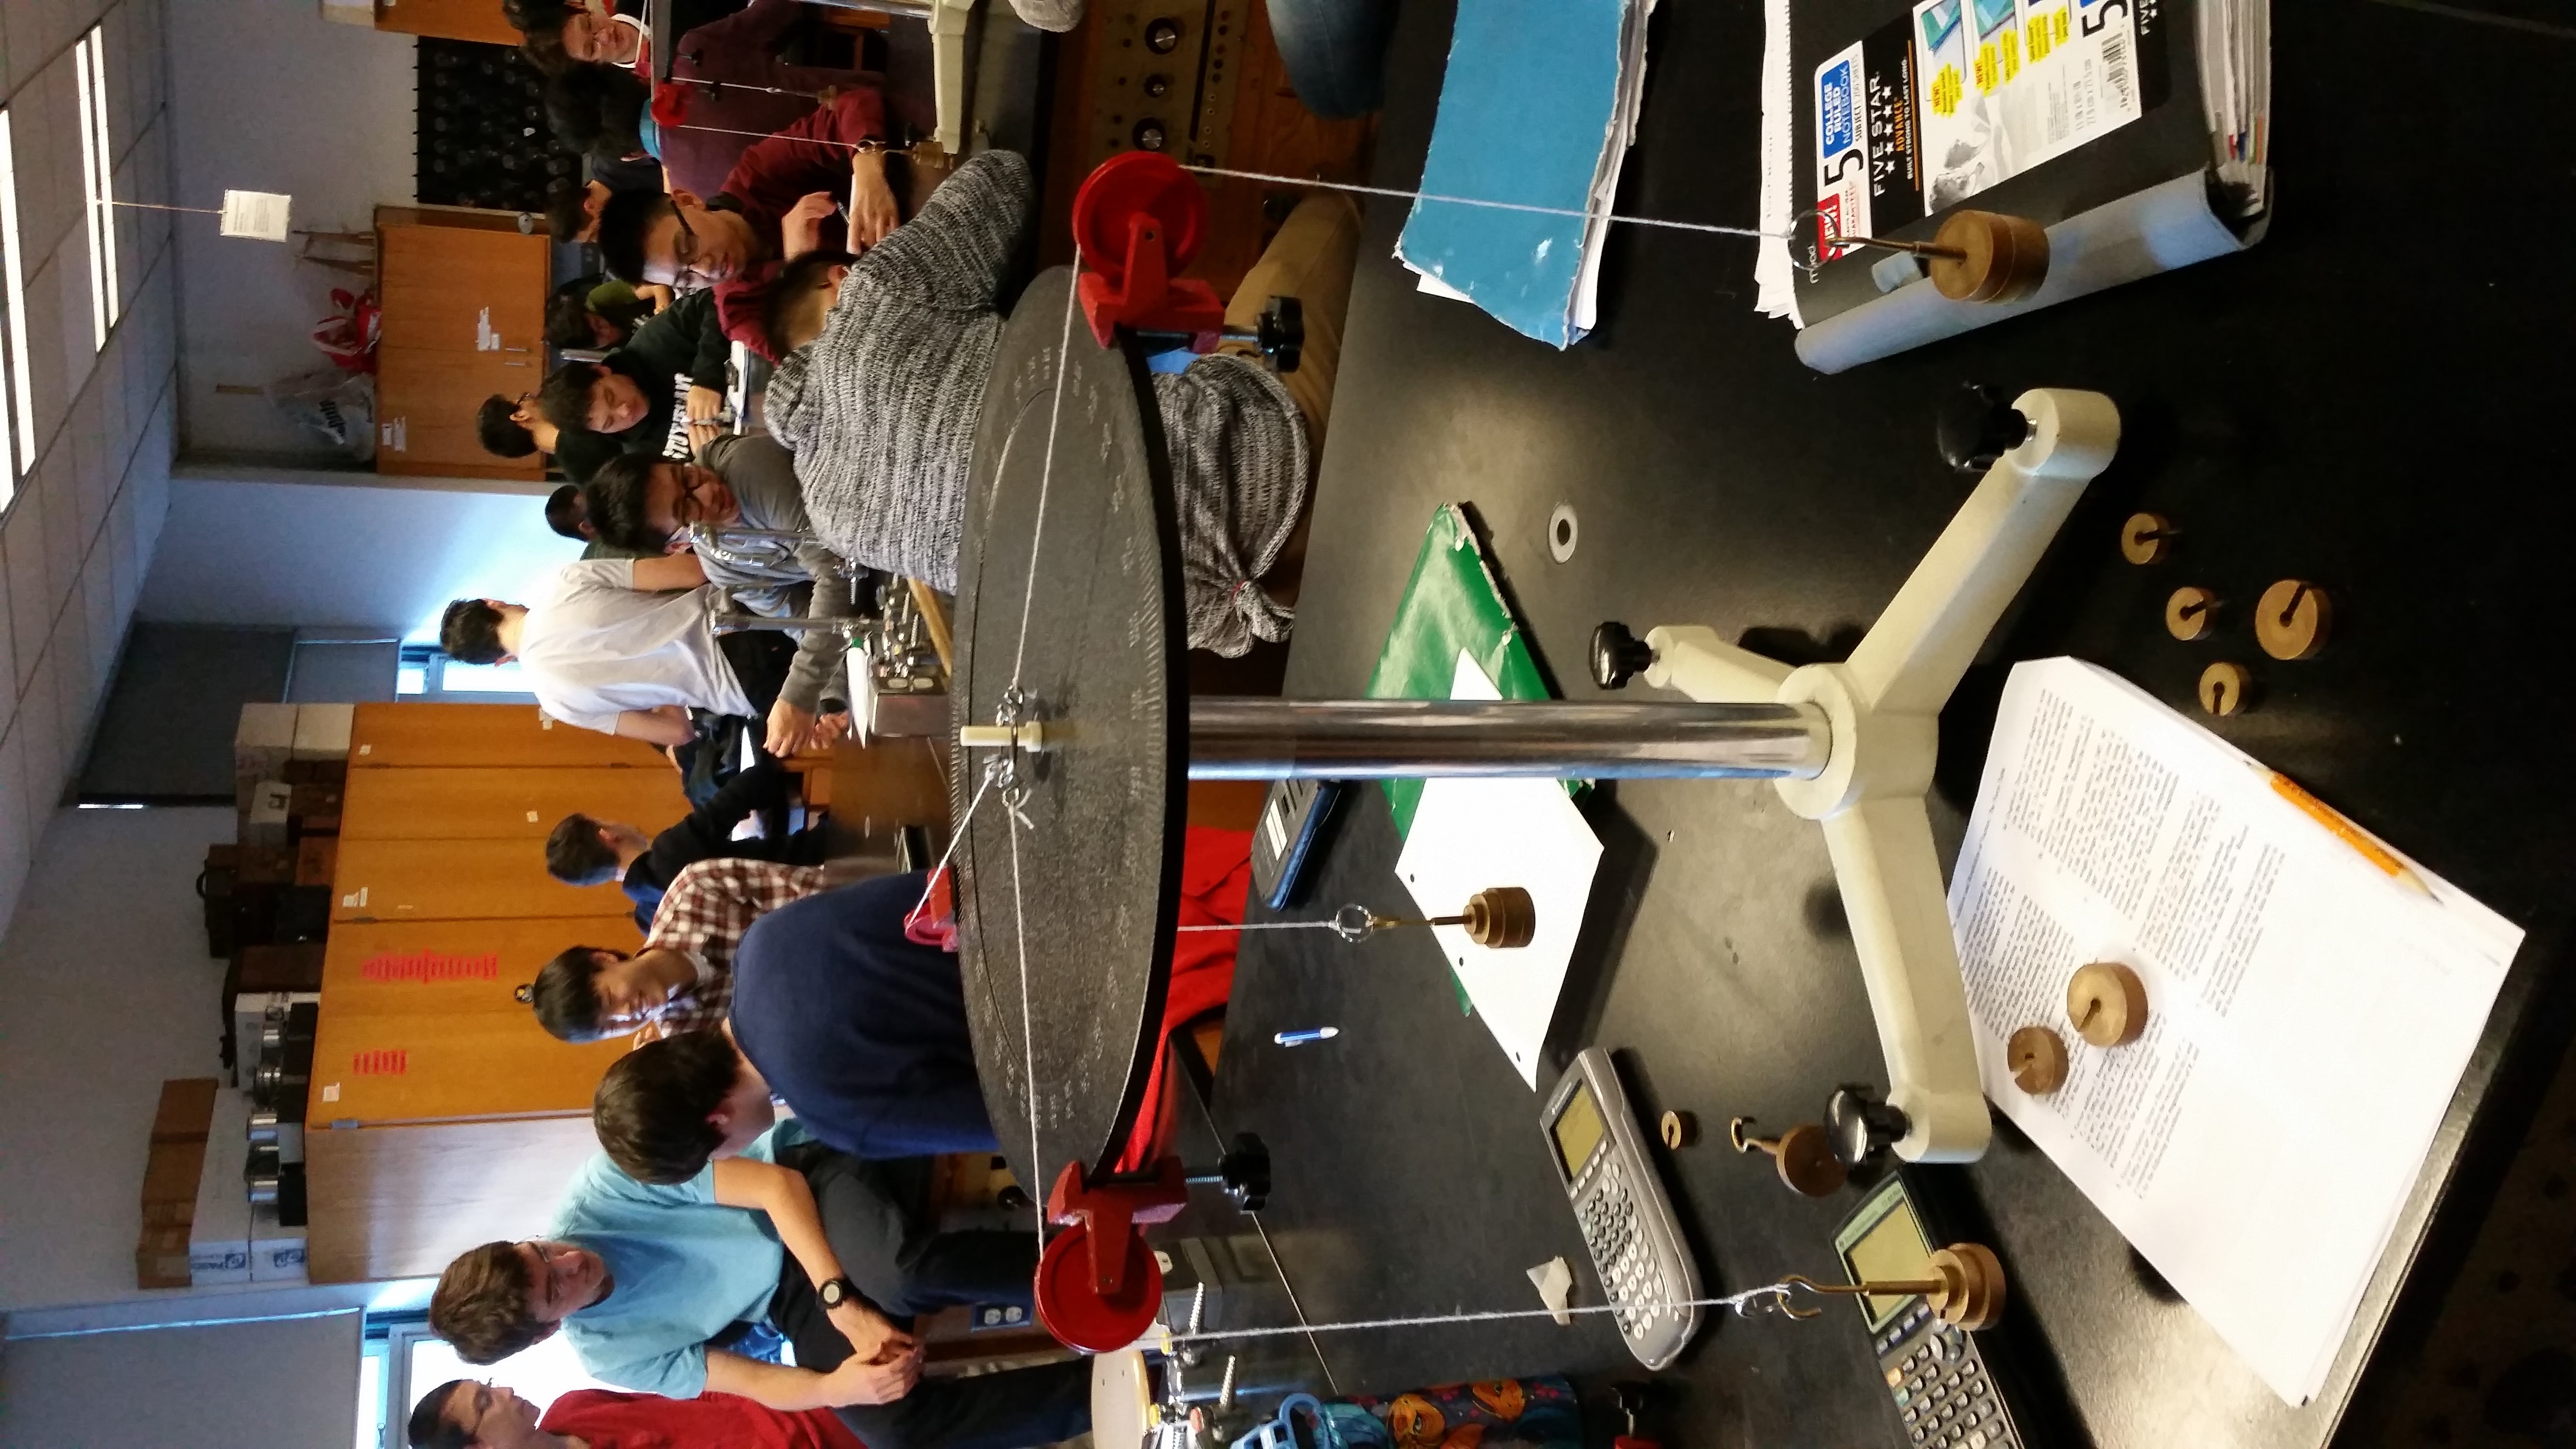
\includegraphics[scale=0.15, angle=270]{lab3.jpg}
\vspace*{17cm}
\end{figure}

\begin{center}
\begin{tabular}
{|m{7em}|m{7em}|m{7em}|m{7em}|m{7em}|}
\hline
Trial & Force Magnitude (N) & Force Angle ($\theta$) & Equilibriant Magnitude (N) & Equilibriant Angle (^o) \\
\hline
Vector Addition 1 & $F_1 = 0.2g, F_2 = 0.2g$ & $\theta_1 = 30^o, \theta_2 = 120^o$ & 0.28g & $255^o$ \\
\hline
Vector Addition 2 &$F_1 = 0.2g, F_2 = 0.15g$ & $\theta_1 = 20^o, \theta_2 = 80^o$ & 0.3g & $225.5^o$ \\
\hline
Vector Addition 3 &$F_1 = 0.2g, F_2 = 0.15g$ & $\theta_1 = 0^o, \theta_2 = 90^o$ & 0.25g & $218^o$ \\
\hline
Vector Resolution &$F = 0.3g$ & $\theta_1 = 60^o$ & $F_x = 0.15g, F_y = 0.26g$ & $\theta_x = 180^o, \theta_y = 270^o$ \\
\hline
Vector Addition 4 &$F_1 = 0.1g, F_2 = 0.2g, F_3 = 0.3g$ & $\theta_1 = 30^o, \theta_2 = 90^o, \theta_3 = 225^o$ & 0.12g & $336^o$ \\
\hline
\end{tabular}
\end{center}

\section*{Discussion}

%\begin{figure}[p]
%\centering
%\hspace*{-10.5cm}
%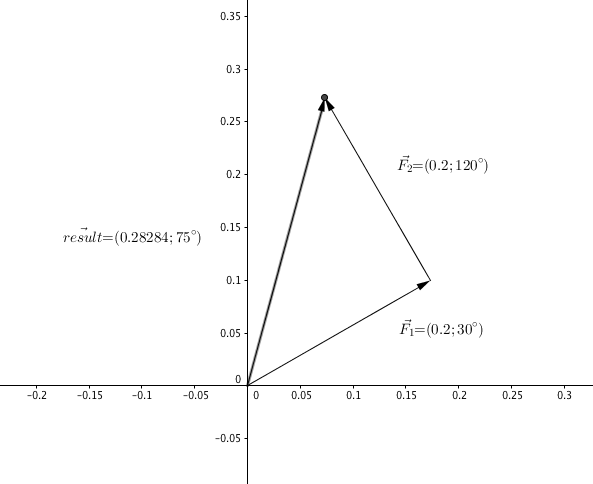
\includegraphics[scale=1.2, angle=0]{vector1.jpg}
%\vspace*{4cm}
%\end{figure}
%\newline
%\begin{figure}[p]
%\centering
%\hspace*{-10.5cm}
%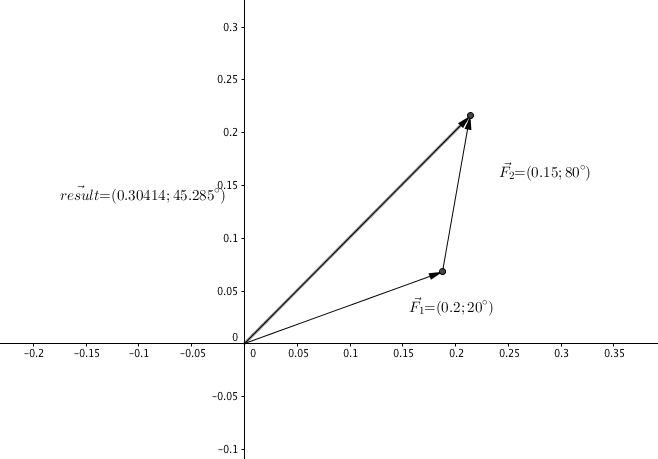
\includegraphics[scale=1.2, angle=0]{vector2.jpg}
%\vspace*{4cm}
%\end{figure}
%\newline
%\begin{figure}[p]
%\centering
%\hspace*{-10.5cm}
%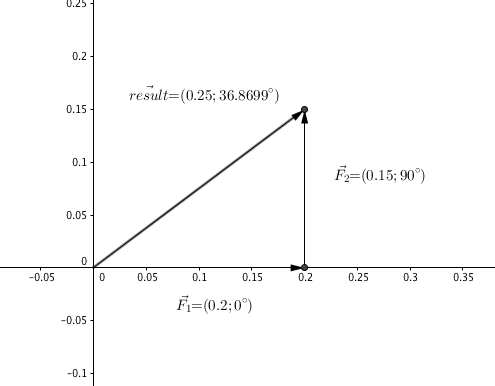
\includegraphics[scale=1.2, angle=0]{vector3.jpg}
%\vspace*{4cm}
%\end{figure}
%\newline
%\begin{figure}[p]
%\centering
%\hspace*{-10.5cm}
%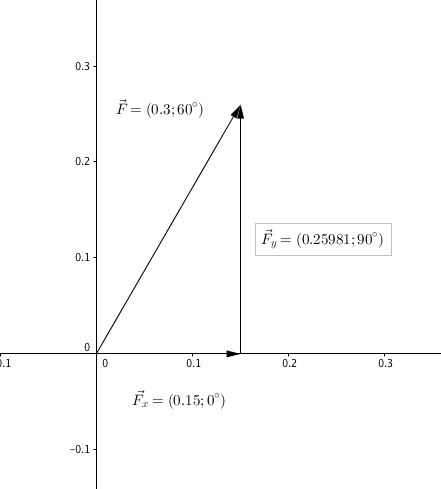
\includegraphics[scale=1.2, angle=0]{vector4.jpg}
%\vspace*{4cm}
%\end{figure}
%\newline
%\begin{figure}[p]
%\centering
%\hspace*{-10.5cm}
%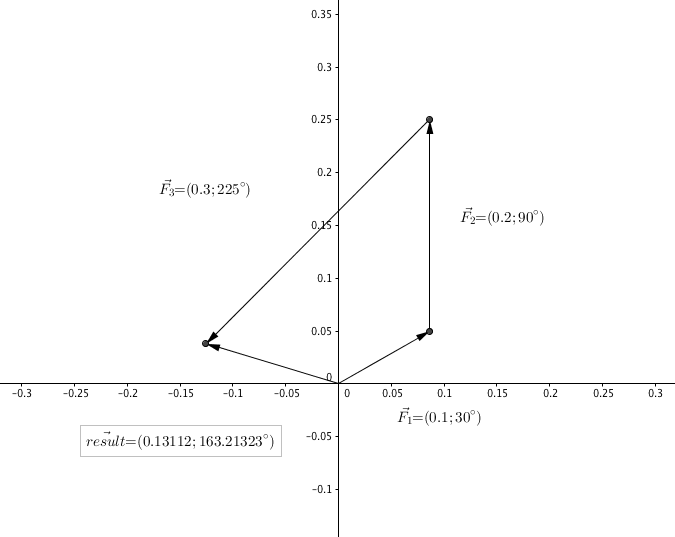
\includegraphics[scale=1.2, angle=0]{vector5.jpg}
%\vspace*{4cm}
%\end{figure}

\begin{center}
\begin{tabular}
{|m{7em}|m{7em}|m{7em}|m{7em}|}
\hline
Trial & Resultant Angle (^o) & Analytical Magnitude (N) & Analytical Angle (^o) \\ 
\hline
Vector Addition 1 & 75 & 0.2828g & 75 \\
\hline
Vector Addition 2 & 45.5 & 0.304g & 45.285 \\
\hline
Vector Addition 3 & 38 & 0.25g & 36.87 \\
\hline
Vector Resolution & $\theta_x = 0^o, \theta_y = 90^o$ & $F_x = 0.15, F_y = 0.2598$ & $\theta_x = 0, \theta_y = 90$ \\
\hline
Vector Addition 4 & 156 & 0.1311g & 163.21 \\
\hline
\end{tabular}
\end{center}

Sample calculations for the non-measured data are as shown for Addition 1:
$$F_{1x} = F_1*cos(\theta_1) = 0.2g*cos(30^o) = 0.1732g N$$
$$F_{1y} = F_1*sin(\theta_2) = 0.2g*sin(30^o) = 0.1g N$$
$$\theta_{result1} = |\theta_{equil1} - 180^o| = |255^o - 180^o| = 75^o$$
$$F_{resultx} = F_{1x} + F{2x} = 0.1732g + -0.1g = 0.0732g N$$
$$F_{result} = \sqrt(F_x^2 + F_y^2) = \sqrt((0.0732g)^2 + (0.2732g)^2) = 0.2828g N$$
$$\theta_{result} = tan^{-1}(\frac{F_y}{F_x}) = tan^{-1}(\frac{0.2732g}{0.0732g}) = 75^o$$

The data gained by the analytical and graphical methods are equal, due to the mathematical form being a representation of the measurements on the graph. The experimental form was very close to the other forms, with slight errors due to issues with measurement and the imprecise nature of the force table, but are very close to the calculated values.

\section*{Conclusion}
The vector addition 1 test measured 0.28g with 75 degrees, rather than the exact 0.2828g with 75 degrees. The vector addition 2 test measured 0.3g with 45.5 degrees, rather than the exact 0.304g with 45.285 degrees. The vector addition 3 test measrued 0.25g with 38 degrees, rather than the exact 0.25g with 36.87 degrees. The vector resolution test measured an x vector of 0.15g and a y vector of 0.26g, rather than the exact 0.15g x vector and 0.2598g y vector. The vector addition 4 measured a 0.12g at 156 degrees vector, rather than the exact 0.1311g with 163.21 degrees vector.  

\end{document}
